\documentclass[a4paper,12pt]{jarticle}
\usepackage[dvipdfmx]{graphicx}
\usepackage{amsmath}
\usepackage{subfigure}
\usepackage{comment}

\setlength{\hoffset}{0cm}
\setlength{\oddsidemargin}{-3mm}
\setlength{\evensidemargin}{-3cm}
\setlength{\marginparsep}{0cm}
\setlength{\marginparwidth}{0cm}
\setlength{\textheight}{24.7cm}
\setlength{\textwidth}{17cm}
\setlength{\topmargin}{-45pt}

\renewcommand{\baselinestretch}{1.6}
\renewcommand{\floatpagefraction}{1}
\renewcommand{\topfraction}{1}
\renewcommand{\bottomfraction}{1}
\renewcommand{\textfraction}{0}
\renewcommand{\labelenumi}{(\arabic{enumi})}
%\renewcommand{\figurename}{Fig.} %図をFig.にする

%図のキャプションからコロン:を消す
\makeatletter
\long\def\@makecaption#1#2{% #1=図表番号、#2=キャプション本文
\sbox\@tempboxa{#1. #2}
\ifdim \wd\@tempboxa >\hsize
#1 #2\par 
\else
\hb@xt@\hsize{\hfil\box\@tempboxa\hfil}
\fi}
\makeatother
% 

\title{電機システム制御特論 \ レポート課題\\
Assignment(2016/06/03)\
}
\author{\vspace{40mm}\\
九州工業大学大学院 \hspace{0mm} 工学府\\
機械知能工学専攻\ \hspace{0mm} 知能制御工学コース \\
\vspace{5mm}\\
所属:\ 西田研究室\\
学籍番号:\ 16344217\\
提出者氏名:\ 津上 \hspace{0mm} 祐典\\\vspace{5mm}\\ }
\date{平成28年\ 6月\ 10日}

\begin{document}

%表紙
\titlepage
\maketitle

\newpage

\thispagestyle{empty}
\tableofcontents

\newpage
\setcounter{page}{1}
%%%%%%%%%%%%%%%%%%%%%%%%
\section{問題}
%%%%%%%%%%%%%%%%%%%%%%%%
以下に示す特性を持つDCモータの速度制御系を少なくとも2つの方法で設計せよ.
%
\begin{table}[h]
 \centering
 \caption{DCモータのパラメータ}
 \label{table:DC_dim}
 \begin{tabular}{c|c|c} \hline
  名称 [単位]                    & 記号  & 数値\\\hline
  定格電力 [kW]                  &$P$    &150  \\\hline
  定格電圧 [V]                   &$V$    &450  \\\hline
  電機子抵抗 [$\Omega$]          &$R_a$  & 0.15 \\\hline
  電機子インダクタンス [H]        &$L_a$   &0.003\\\hline
  慣性モーメント [kg$\rm {m^3}$] &$J$     &10  \\\hline
  誘起電圧定数 [V$\cdot$s/rad]    &$K_E$   &8.50 \\\hline
  トルク定数 [Nm/A]               & $K_T$  &8.50 \\\hline
  基底速度 [rpm]                &$\omega$&500  \\\hline
 \end{tabular}
\end{table}
%
%%%%%%%%%%%%%%%%%%%%%%%%%
\section{DCモータの特性}
%%%%%%%%%%%%%%%%%%%%%%%%%
はじめに,本レポートで用いるDCモータのブロック線図を図\ref{fig:DC_model}に示す.
%
\begin{figure}[bp]
 \begin{center}
  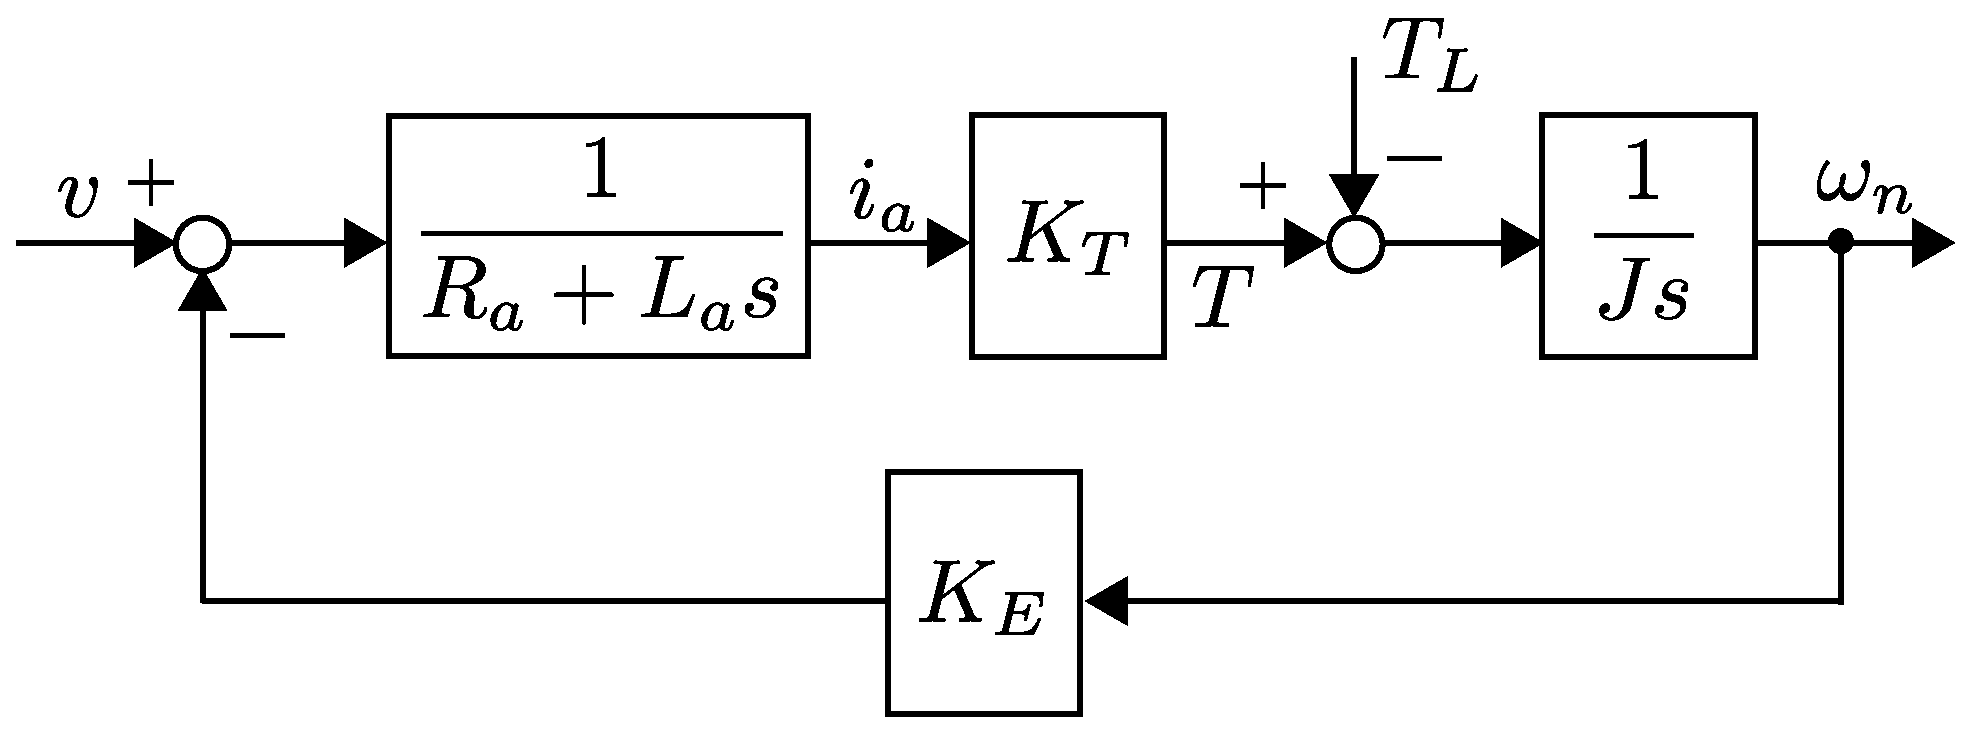
\includegraphics[width = 150mm]{fig/DC_model.eps}
 \end{center}
 \caption{DCモータのブロック線図}
 \label{fig:DC_model}
\end{figure}
%
\newpage
%
はじめに,図\ref{fig:DC_model}に示すDCモータのモデルの伝達特性を導出する.
図\ref{fig:DC_model}より
%
\begin{equation}
 \Omega_m(s)=\frac{1}{Js}\left\{\frac{K_T}{R_{a}+L_{a}s}(V-K_E\Omega_m)-T_L\right\}
\end{equation}
と表され,式変形すると,
\begin{equation*}
 \left(Js+\frac{K_{T}K_{E}}{R_{a}+L_{a}}s\right)\Omega_m(s)=\frac{K_{T}}{R_{a}+L_{a}s}-T_L
\end{equation*}
%
\begin{equation*}
 \Omega_m(s)=\frac{K_T}{JL_{a}s^2+JR_{a}s+K_TK_E}-\frac{R_{a}+L_{a}s}{JL_{a}s^2+JR_{a}s+K_TK_E}T_L
\end{equation*}
%
\begin{equation}
 \Omega_m(s)=\frac{\frac{1}{K_E}}{\frac{JL_a}{K_{T}K_E}s^2+\frac{JR_a}{K_{T}K_E}s+1}-\frac{\frac{R_{a}+L_{a}s}{K_{T}K_E}}{\frac{JL_a}{K_{T}K_E}s^2+\frac{JR_a}{K_{T}K_E}s+1}T_L
\end{equation}
%
となる.(2)式において
\begin{eqnarray}
 \begin{cases}
  T = \sqrt{\frac{L_{a}J}{K_{E}K_T}} & \\
  \zeta= \frac{R_a}{2}\sqrt{\frac{J}{K_{E}K_{T}L_a}} & \\
  K = \frac{1}{K_E}
 \end{cases}
\end{eqnarray}
とおく.負荷を含まないDCモータ単体の入出力伝達関数$P(s)$は,
\begin{equation}\label{equ:plant}
 P(s)=\frac{K}{T^2s^2+2\zeta Ts+1}
\end{equation}
となる.
%
%%%%%%%%%%%%%%%%%%%%%%%%%
\section{I-PD制御}
%%%%%%%%%%%%%%%%%%%%%%%%%
本節ではをI-PD制御によるDCモータの速度制御系を設計する.

%%%%%%%%%%%%%%%%%%%%%%%%%
\subsection{I-PD制御の原理}
%%%%%%%%%%%%%%%%%%%%%%%%%
はじめにI-PD制御の原理について説明する.一般的なPID制御系の構造は直列補
償型であるのに対してI-PD制御系の構造は
直列補償+フィードバック補償型である.PID制御系に目標値として
ステップ関数が入力されたとき,制御入力$u$は微分要素によってデルタ関数を
含む形になる.これは微分キックと呼ばれ,システム機器が危険な状態になる可
能性がある.これを避けるためにPIDコントローラの微分要素をフィードバッ
クパスに移動させた制御系をPI-D制御系と呼ぶ.さらに,ステップ状の制御入力
を妨げるために比例要素をフィードバックパスに移動させた制御系が本節で取り
扱うでI-PD制御系である.図\ref{fig:IPD_b}にI-PD制御系の
ブロック線図を示す.
%
\begin{figure}[bp]
 \begin{center}
  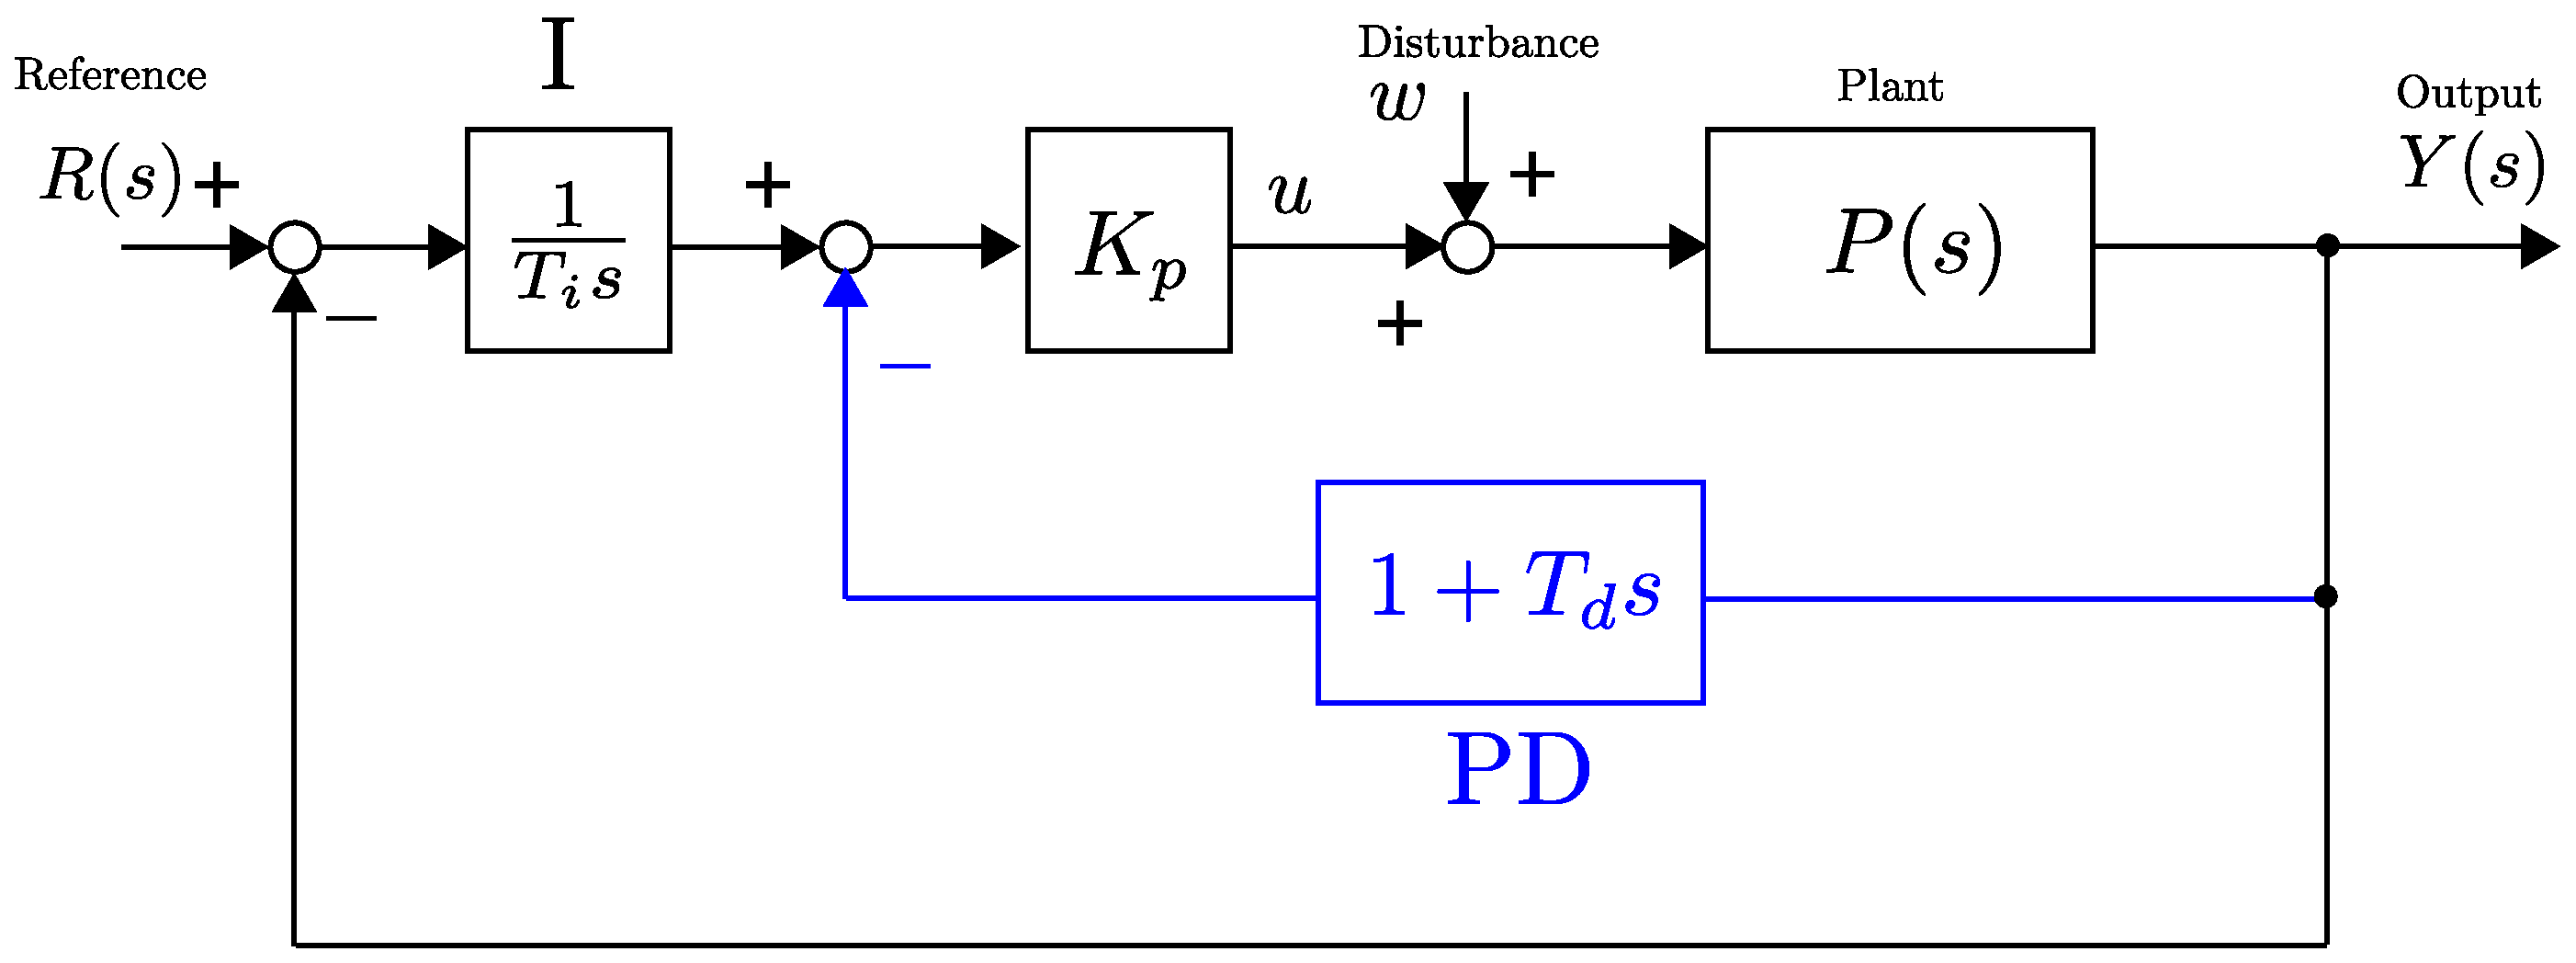
\includegraphics[width = 150mm]{fig/IPD_b.eps}
 \end{center}
 \caption{I-PD制御系}
 \label{fig:IPD_b}
\end{figure}
%
ここで,
%
\begin{equation}
 \frac{K_i}{s} = \frac{K_p}{T_is} \ \ , \ \ F(s) = K_p(1+T_d s)
\end{equation}
%
とおくと,図\ref{fig:IPD_b}は図\ref{fig:IPD_a}のように表せる.
%
\begin{figure}[tbp]
  \begin{center} 
  \subfigure[IP-D]{
    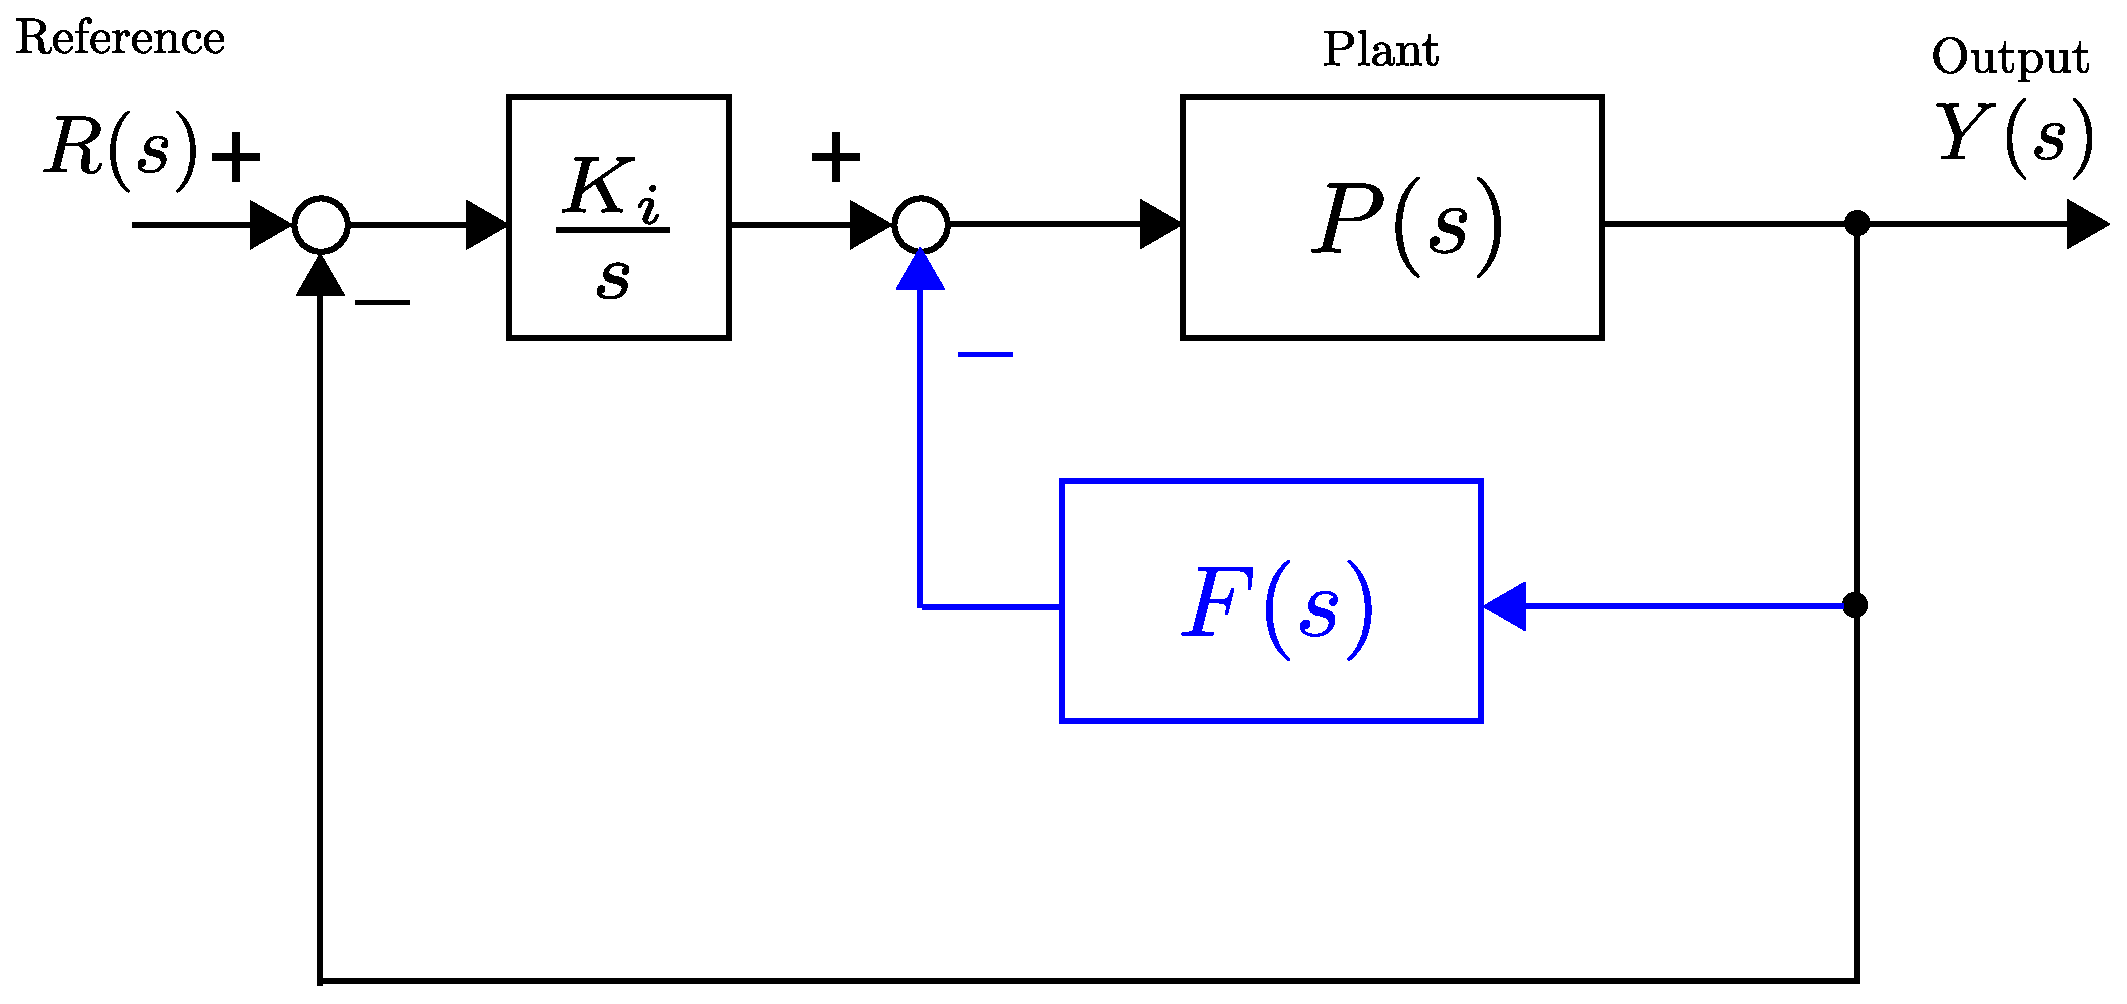
\includegraphics[width = 90 mm]{fig/IPD_a.eps}
     \label{fig:IPD_a}
  }
  %
  \hfill
  %
  \subfigure[reference model]{
   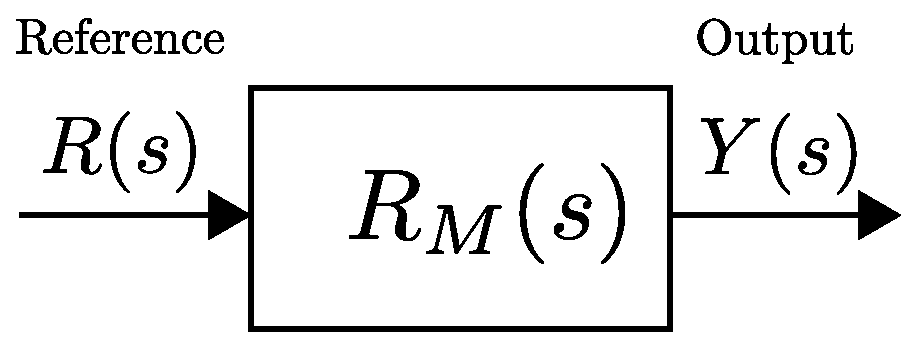
\includegraphics[width = 70mm]{fig/IPD_r.eps}
    \label{fig:IPD_r}
  }
  \end{center}
  \caption{I-PD制御系の設計}
  \label{fig:IPD}
\end{figure}
%
図\ref{fig:IPD_r}に示すようなI-PD制御系の伝達関数と等しい参照モデル$R_M(s)$を決定
する.3次系の$R_M(s)$は,
%
\begin{equation}\label{equ:R_M}
 R_M(s) = \frac{1}{\alpha_0+\alpha_1\sigma s+\alpha_2 (\sigma s)^2+\alpha_3(\sigma s)^3}
\end{equation}
%
と表現できる.ただし,$\sigma$はタイムスケールを表す.また,
$\left\{\alpha_0,\alpha_1,\alpha_2,\alpha_3\right\}=\left\{1,1,0.5,0.15\right\}$と北森は推薦してい
る.ここで図\ref{fig:IPD_a}より$R(s),Y(s)$の関係を求めると,
%
\begin{equation}
 Y(s) = P(s)\left\{\frac{K_i}{s}(R(s)-Y(s))-F(s)Y(s) \right\}
\end{equation}
%
となる.すると伝達関数$T(s)$,
%
\begin{equation}
 T(s) = \frac{Y(s)}{R(s)} =
  \frac{\frac{K_i}{s}P(s)}{1+P(s)\Bigl(\frac{K_i}{s}+F(s)\Bigr)} =  \frac{1}{1+\frac{s}{K_i}\Bigl(\frac{1}{P(s)}+F(s)\Bigr)}
\end{equation}
%
を得る.ここでプラント$P(s)$が2次系で
%
\begin{equation}\label{equ:beta}
 P(s) = \frac{1}{\beta (s)} = \frac{1}{\beta_0 + \beta_1 s + \beta_2 s^2}
\end{equation}
%
と表現されるとき,I-PDコントローラのパラメータは,
%
\begin{eqnarray}
 T(s) & = & R_M(s) \nonumber \\
 \frac{1}{1+\frac{s}{K_i}\Bigl(\beta_0 + \beta_1 s + \beta_2 s^2 +
  K_p+K_p T_d s \Bigr)} & = & \frac{1}{\alpha_0+\alpha_1\sigma
  s+\alpha_2 (\sigma s)^2+\alpha_3(\sigma s)^3} \nonumber \\
 \frac{1}{1+\frac{\beta_0 + K_p}{K_i}s+\frac{K_pT_d+_beta_1}{K_i}s^2+\frac{\beta_2}{K_i}s^3}& = & \frac{1}{\alpha_0+\alpha_1\sigma s+\alpha_2 (\sigma s)^2+\alpha_3(\sigma s)^3}\label{equ:equal}
\end{eqnarray}
%
より決定できる.
%
%%%%%%%%%%%%%%%%%%%%%%%%%
\subsection{I-PD制御による制御系の設計}
%%%%%%%%%%%%%%%%%%%%%%%%%
次に,先ほど説明したIP-D制御を用いてDCモータの速度制御系を設計する.
はじめに,参照モデル$R_M(s)$中の$\sigma=1,2,3$としたときの場合のステップ
応答を図\ref{fig:IPDr}に示す.ただし,$\alpha_i(i=9,1,2,3)$は北森の推薦
する
$\left\{\alpha_0,\alpha_1,\alpha_2,\alpha_3\right\}=\left\{1,1,0.5,0.15\right\}$
を用いた.
%
\begin{figure}[tbp]
 \begin{center}
  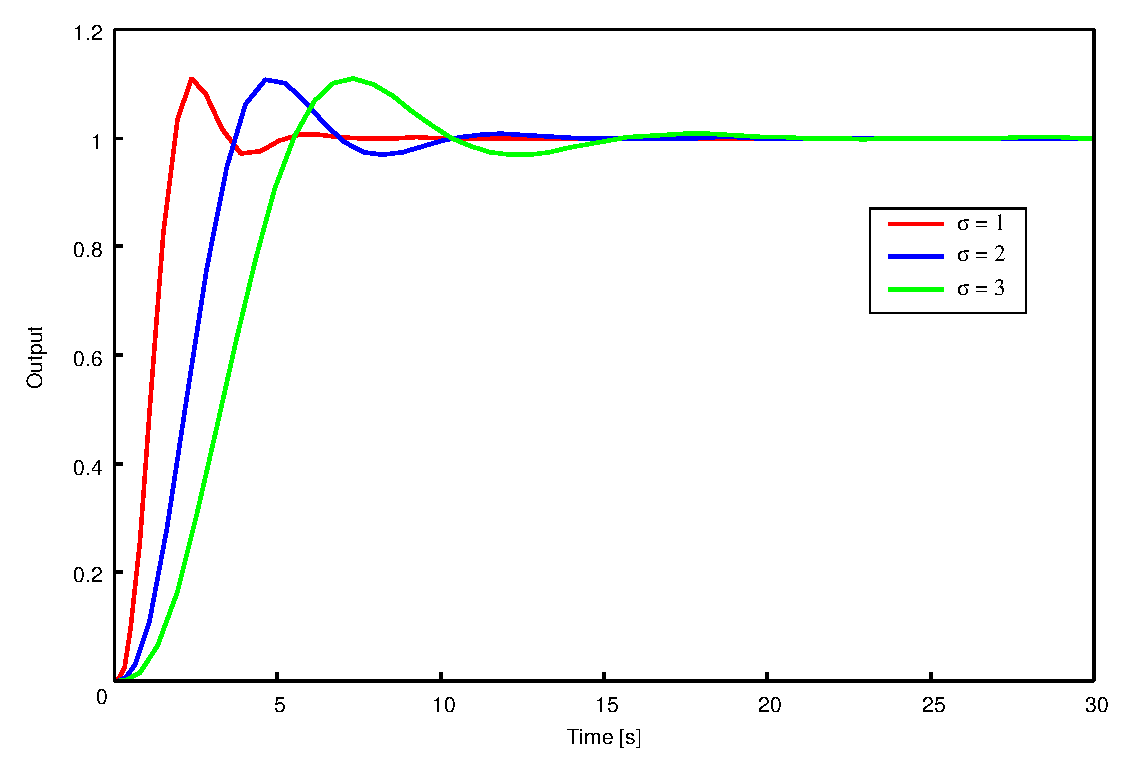
\includegraphics[width = 150mm]{fig/IPDr.eps}
 \end{center}
 \caption{参照モデル$R_M(s)$のステップ応答}
 \label{fig:IPDr}
\end{figure}
%
図\ref{fig:IPDr}より,********であるから$\sigma=1$を採用した.
次に,(\ref{equ:beta})式の$\beta_i(i=0,1,2)$を具体的に計算すると,
%
\begin{eqnarray}
 \begin{cases}
  \beta_0  =  \frac{1}{K} = K_E = 8.50 \\
  \beta_1  =  \frac{2\zeta T}{K} = \frac{R_a J}{K_T} = \frac{3}{17} \\
  \beta_2  =  \frac{T^2}{K} = \frac{L_a J}{K_T} = \frac{3}{850}
 \end{cases}
\end{eqnarray}
%
となる.これらを(\ref{equ:equal})式に代入し,係数比較すると,コントロー
ラのパラメータである
%
\begin{eqnarray}
 \begin{cases}
  K_p = -\frac{1441}{170} \\
  T_d = \frac{28}{1441} \\
  K_i = \frac{2}{85}
 \end{cases}
\end{eqnarray}
%
を得る.
%
%%%%%%%%%%%%%%%%%%%%%%%%%
\subsection{シミュレーションと考察}
%%%%%%%%%%%%%%%%%%%%%%%%%
I-PD制御を用いたDCモータの速度制御系を構成し,
MATLAB/simulinkでシミュレーションを行った.DCモータをI-PD制御したときのステップ応
答と参照モデル$R_M(s)$のステップ応答の比較をしたものを図
\ref{fig:IPD_com}に示す.
%
\begin{figure}[tbp]
 \begin{center}
  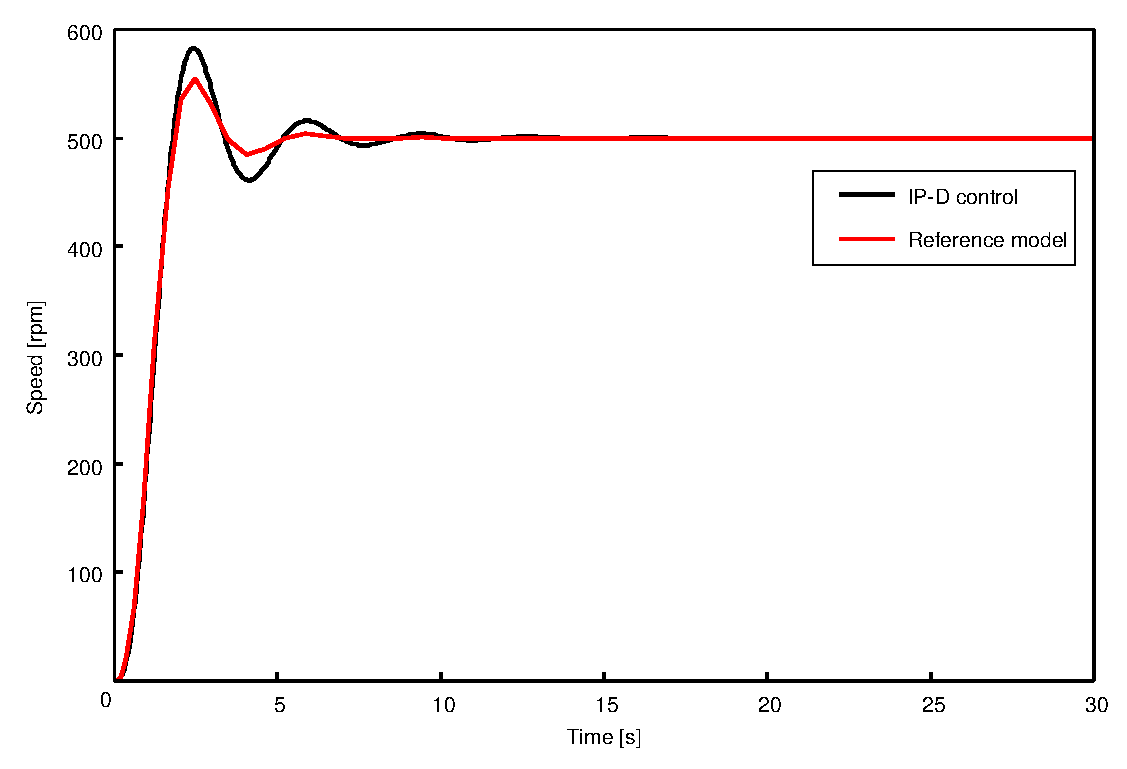
\includegraphics[width = 150mm]{fig/IPD_com.eps}
 \end{center}
 \caption{I-PD制御したときのステップ応答と参照モデル$R_M(s)$のステップ応答の比較}
 \label{fig:IPD_com}
\end{figure}
%

図\ref{fig:IPDr},\ref{fig:IPD_com}を見ると応答波形が振動していることがわ
かる.これは係数$\alpha_i$を望ましいステップ応答形状に応じて適宜変更する
ことで制御可能であると考えられる.
%
I-PD制御系の特徴としてPID制御系より目標値への追従が遅い,また,速応性を上げ
過ぎると制御系が不安定になる場合があることが挙げられる.

\newpage

%%%%%%%%%%%%%%%%%%%%%%%%%
\section{IMC(Internal Model Contorl)法}
%%%%%%%%%%%%%%%%%%%%%%%%%
本節ではIMC(Internal Model Contorl)法を用いてDCモータの速度制御系を設計
する.IMC法(内部モデル制御法)は適切なフィルタを選ぶことで簡単に安定な
制御系を設計できる手法である.
%%%%%%%%%%%%%%%%%%%%%%%%%
\subsection{IMCの原理}
%%%%%%%%%%%%%%%%%%%%%%%%%
まず,IMC法の原理について説明する.
%
\begin{figure}[bp]
 \begin{center}
  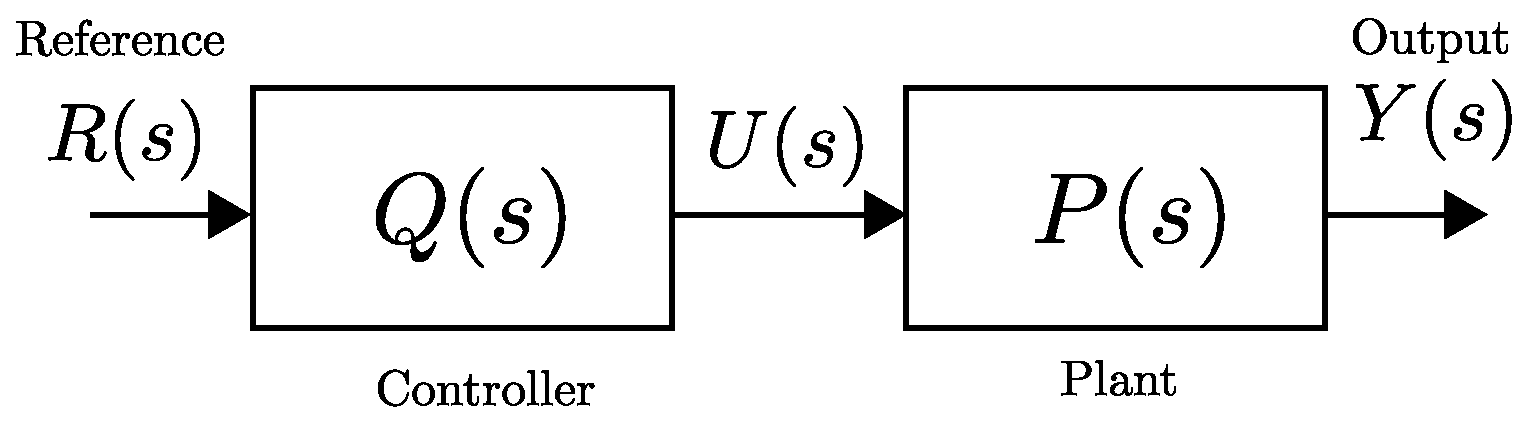
\includegraphics[width = 80mm]{fig/FF.eps}
 \end{center}
 \caption{フィードフォワード制御系}
 \label{fig:ff}
\end{figure}
%
図\ref{fig:ff}にフィードフォワード制御系のブロック線図
を示す.ここで,コントローラ$Q(s)$がプラントのモデル$P(s)$の逆数と等価で
あるとき,出力$Y(s)$は,入力を$R(s)$とすると,
\begin{equation}
Y(s) = P(s)Q(s)R(s) = P(s)P^{-1}(s)R(s) =R(s)
\end{equation}
となる.つまり,出力$Y(s)$は入力$R(s)$と等しくなる.これがIMC法の原理であ
り,コントローラはプラントのモデルの情報を含む形になる.図\ref{fig:IMC}
にIMC法を用いた制御系のブロック線図を示す.
%
\begin{figure}[tbp]
 \begin{center}
  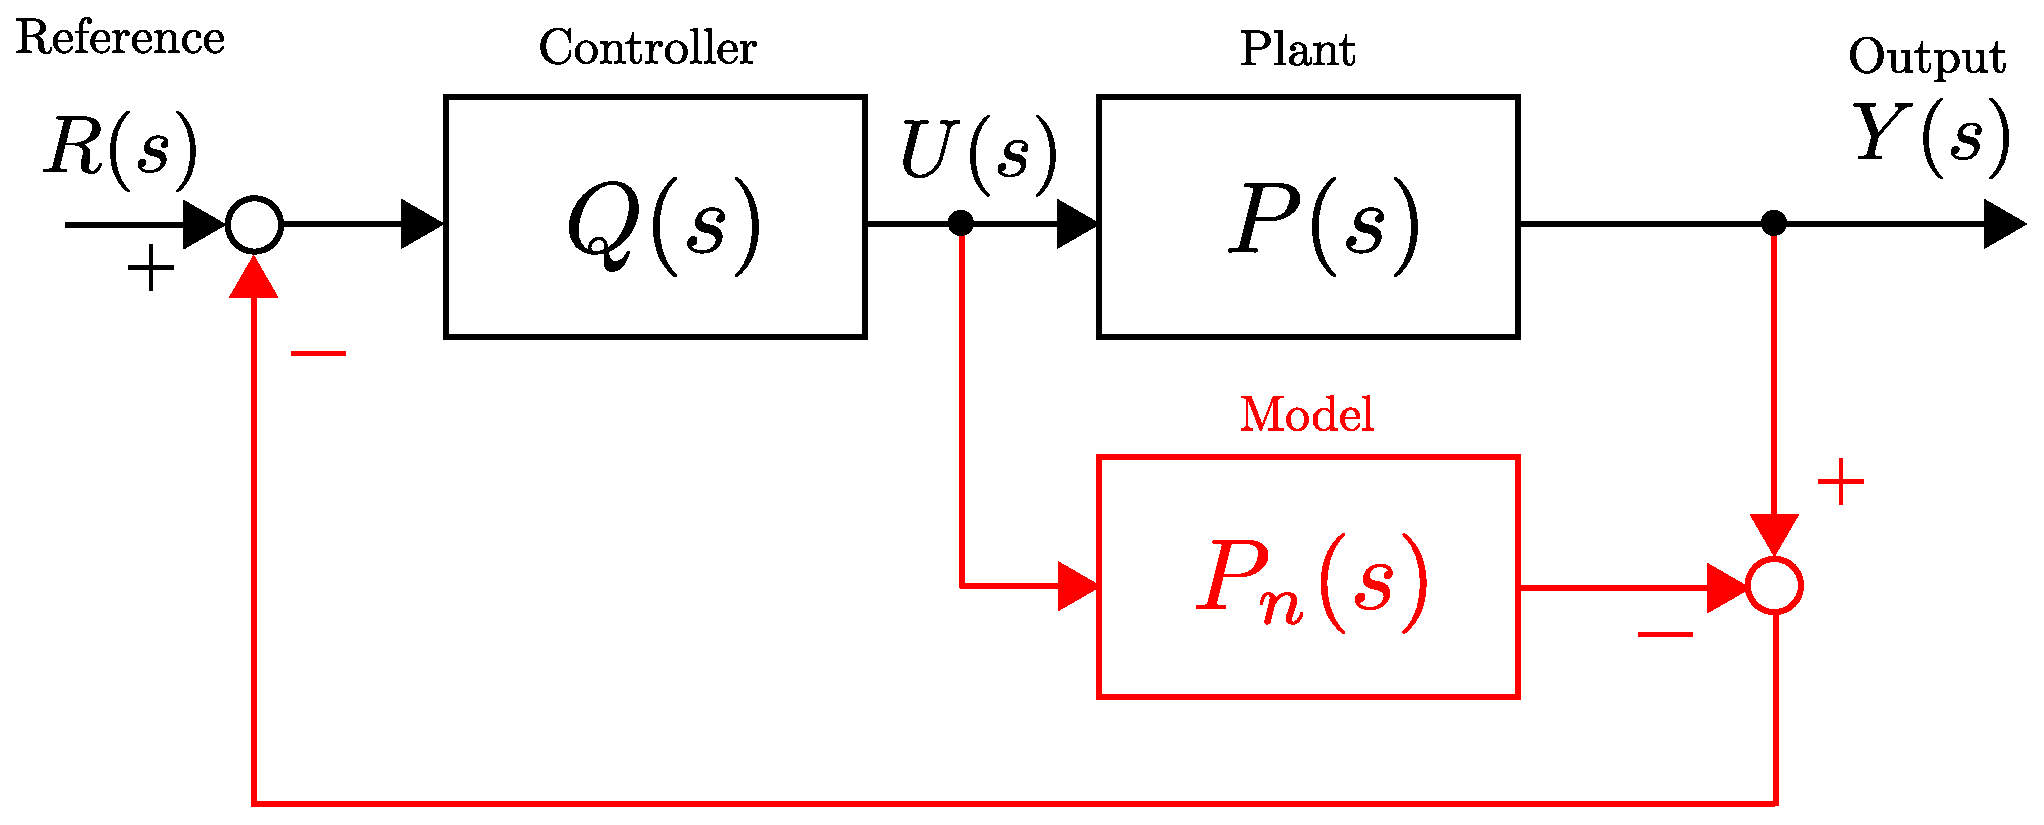
\includegraphics[width = 100mm]{fig/IMC.eps}
 \end{center}
 \caption{IMC法を用いた制御系}
 \label{fig:IMC}
\end{figure}
%
ここで$P_n(s)$はプラントのノミナルモデルである.もし,ノミナルモデルがプ
ラントのモデルと完全に一致(つまり$P_n(s)=P(n)$)しているなら,プラント
の出力とノミナルモデルの出力は等しくなる.したがって,図\ref{fig:ff}に示
すフィードフォワード制御系と等価になる.コントローラはプラントのモデルの
逆数であることが望ましいが,場合によって,右半面に零点(実部が正の零点)もしくはむだ時間要
素を持つシステムである非最小位相(NMP)系になる可能性がある.プラントの
モデルの逆数は制御系のパフォーマンスに影響してくる.このようになった場合
の改善策として以下の3点が挙げられる.
%
\begin{itemize}
 \item プラントにむだ時間要素を含む場合,$P^{-1}(s)$はコントローラとして使えないので
	   $P^{-1}(s)$からむだ時間要素を取り除けば良い(無視すれば良い).
	   
 \item プラントに実部が正の零点を持つ場合,$P^{-1}(s)$は不安定である.こ
	   の場合は,実部が正の零点を取り除き,実部が正の零点を含むよ
	   うな全域通過関数(all-pass function)を構成すれば良い.例として,
	   $P_n(s)$に$s=4$という実部が正の零点を持つ場合,$P_n(s)$に
	   $(s+4)/(s+4)$を掛ける.すると全域通過関数は$(s+4)/(s-4)$となる.
	   
 \item $P(n)$が厳密にプロパーで,$P^{-1}(s)$がプロパーでない場合,IMCフィ
	   ルターと呼ばれるローパスフィルタを追加すれば良い.
\end{itemize}
%
上述した3つ目の場合におけるコントローラの設計に関して考える.プラントの
ノミナルモデル$P_n(s)$は最小位相(Minimum Phase)部$P_{nM}(s)$と全域通過
(all-pass)部$P_{nA}(s)$に分解できる.
%
\begin{equation}
 P_n(s)=P_{nM}(s)P_{nA}(s)
\end{equation}
%
ここで$P_{nA}(s)$はむだ時間要素もしくは実部が正の零点をもつ伝達関数であ
る.ここで,IMCフィルタは以下の式で与えられる.
%
\begin{equation}\label{equ:imc_f}
 F(s) = \frac{1}{(\lambda s + 1)^n}
\end{equation}
%
したがってコントローラ$Q(s)$は
%
\begin{equation}\label{equ:imc_c}
 Q(s) = P_{nM}^{-1}(s)F(s)
\end{equation}
%
となる.また,図\ref{fig:IMC}に示したIMCを用いた制御系は図\ref{fig:henkan}に示すよう
な等価変形することが出来る.
%
\begin{figure}[tbp]
  \begin{center} 
  \subfigure[IMC]{
    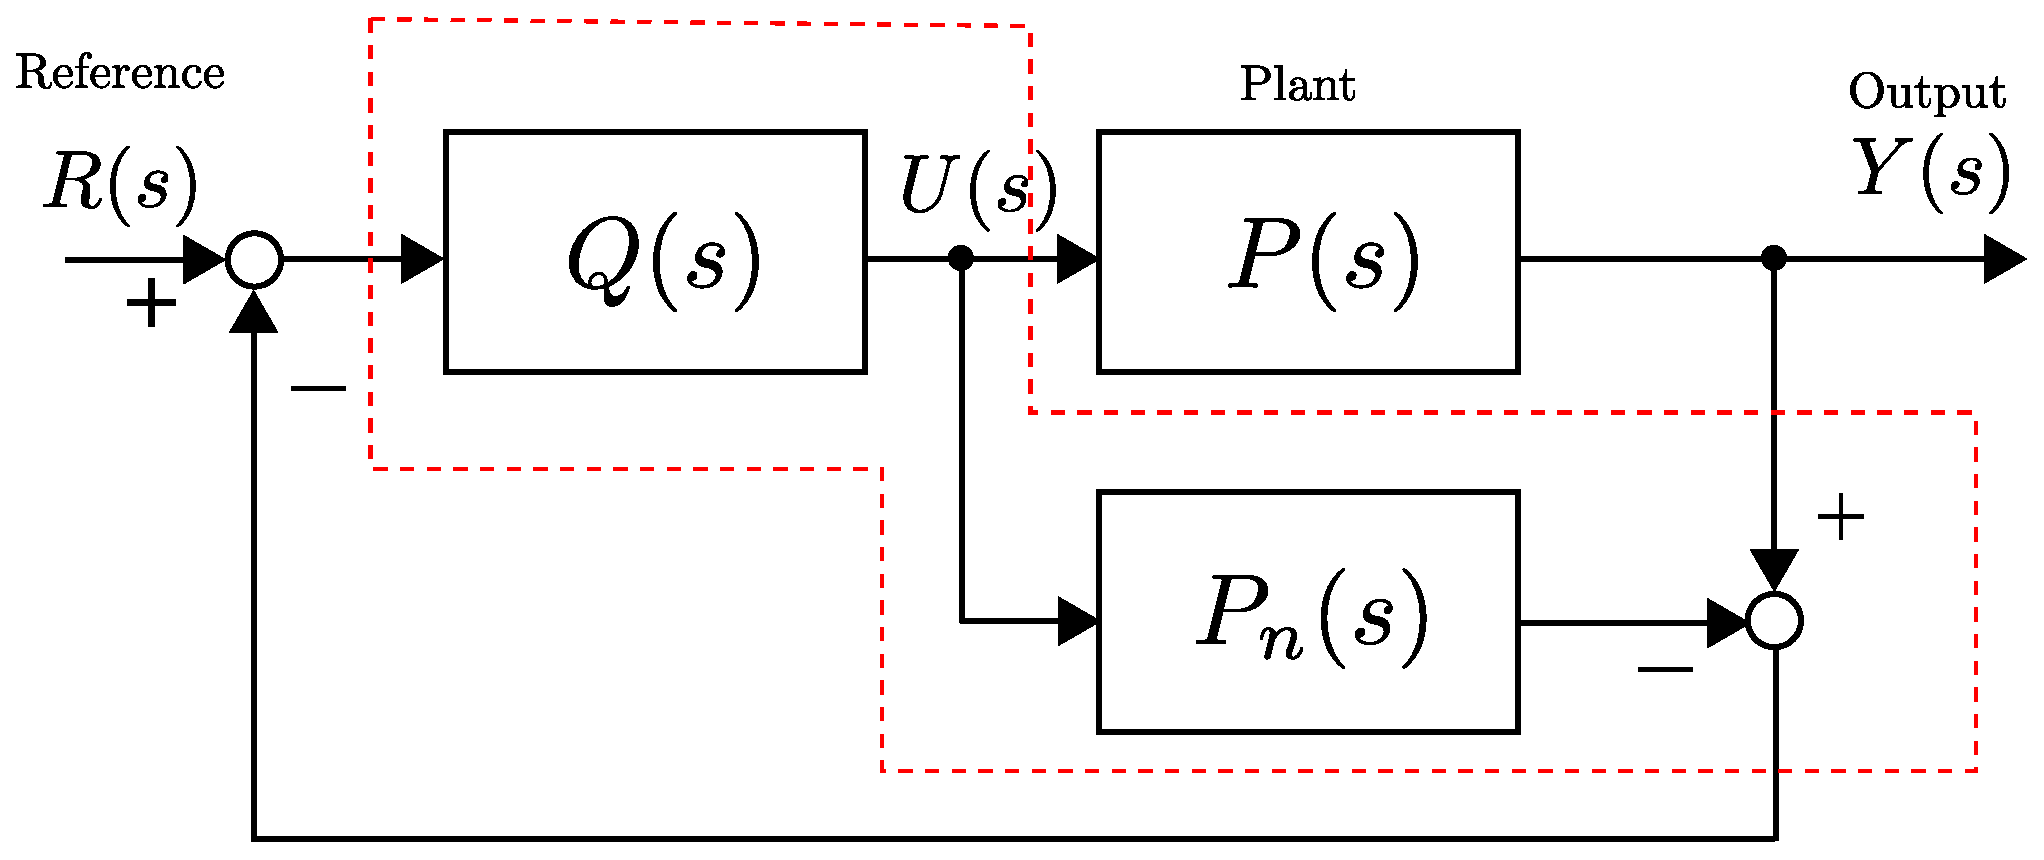
\includegraphics[width = 80 mm]{fig/IMC_a.eps}
     \label{fig:IMC_a}
  }
  %
  \hfill
  %
  \subfigure[IMCを等価変換したもの]{
   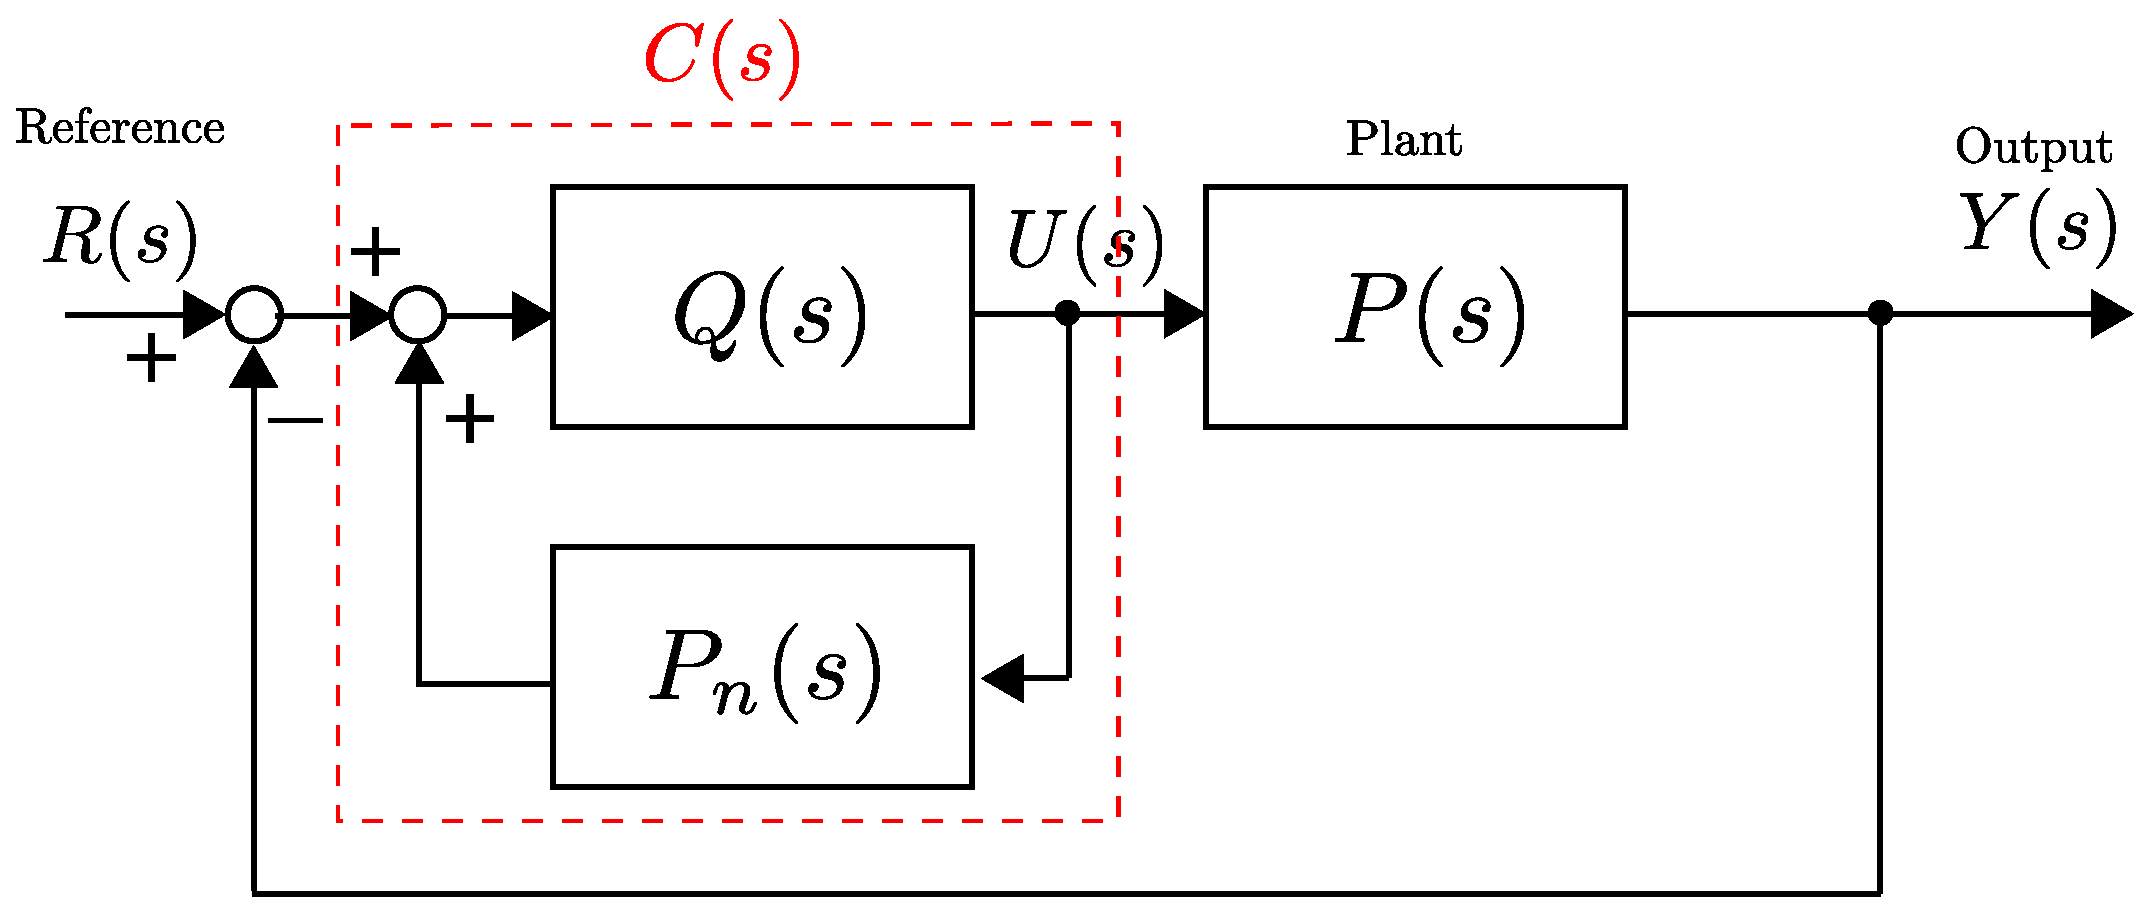
\includegraphics[width = 80mm]{fig/IMC_b.eps}
    \label{fig:IMC_b}
  }
  \end{center}
  \caption{IMCの等価変換}
  \label{fig:henkan}
\end{figure}
%
図\ref{fig:IMC_b}中のコントローラ$C(s)$は,
%
\begin{equation}
 C(s) = \frac{Q(s)}{1 - P_n(s)Q(s)}
\end{equation}
%
となる.
%%%%%%%%%%%%%%%%%%%%%%%%%
\subsection{IMC法によるPIDコントローラの設計}
%%%%%%%%%%%%%%%%%%%%%%%%%
次に,先ほど説明したIMC法を用いてDCモータの速度制御系を設計する.
ここではノミナルモデルはプラントと等しい,つまり$P(s)=P_{n}(s)$である.
また,ノミナルモデルは最小位相系である,つまり$P_n(s)=P_{nM}(s)$であると
仮定する.すると,IMCコントローラ$Q(s)$は(\ref{equ:plant}),(\ref{equ:imc_c})式より
%
\begin{equation}
 Q(s) = P_{nM}^{-1}(s)F(s) = P^{-1}(s)F(s) = \frac{T^2s^2+2\zeta Ts+1}{K}F(s) 
\end{equation}
%
となる.ここで一次($n=1$)のIMCフィルタ$F(s)$を考えると,
(\ref{equ:imc_f})式より$F(s)$は
%
\begin{equation}
 F(s) = \frac{1}{\lambda s + 1}
\end{equation}
%
となる.以上より,IMCコントローラ$Q(s)$は
%
\begin{equation}
 Q(s) = \frac{T^2s^2+2\zeta Ts+1}{K(\lambda s + 1)}
\end{equation}
%
となる.したがって,一般のフィードバックコントローラ$C(s)$は
%
\begin{eqnarray}\label{equ:C_s}
 C(s) & = & \frac{Q(s)}{1 - P_n(s)Q(s)} \nonumber  \\ 
  & = & \frac{\frac{T^2s^2+2\zeta Ts+1}{K(\lambda s +
  1)}}{1-\frac{K}{T^2s^2+2\zeta Ts+1}\frac{T^2s^2+2\zeta Ts+1}{K(\lambda
  s + 1)}} \nonumber \\ 
 & = & \frac{T^2s^2+2\zeta Ts+1}{K\lambda s} \nonumber  \\
  & = & \frac{2\zeta T}{K\lambda}\Bigl(1+\frac{1}{2\zeta Ts}+\frac{T}{2\zeta}s\Bigr)
\end{eqnarray}
%
となる.(\ref{equ:C_s})式はPIDコントローラの式
%
\begin{equation}\label{equ:PID}
 C_{PID} (s) = K_p \Bigl(1+\frac{1}{T_i s} + T_d s\Bigr)
\end{equation}
%
と等価であるとみなせる.(\ref{equ:C_s}),(\ref{equ:PID})式を係数比較する
ことによって,
%
\begin{equation}\label{equ:gain}
 K_p =  \frac{2\zeta T}{K\lambda}  \ \  ,  \ \ T_i = 2\zeta T  \ \  , \ \ T_d = \frac{T}{2\zeta}
\end{equation}
%
を得る.$\lambda$の値を任意に3つ決定し,(\ref{equ:gain})式に具体的な値を
代入したものを表\ref{tab:IMC_para}に示す.
%
\begin{table}[tb]
 \centering
 \caption{IMC法を用いて決定したPIDパラメータ}
 \label{tab:IMC_para}
  \begin{tabular}{c||c|c|c}\hline
       \        &$K_p$  &$T_i$   &$T_d$\\\hline
   $\lambda=0.1$&1.765  &0.020761&0.02\\\hline
   $\lambda=0.2$&0.88235&0.020761&0.02\\\hline
   $\lambda=0.5$&0.35294&0.020761&0.02\\\hline
 \end{tabular}
\end{table}
%
%%%%%%%%%%%%%%%%%%%%%%%%%
\subsection{シミュレーションと考察}
%%%%%%%%%%%%%%%%%%%%%%%%%
IMC法を用いて決定したPIDコントローラを用いてDCモータの速度制御系を構成し,
MATLAB/simulinkでシミュレーションを行った.このときのシミュレーション結
果を図\ref{fig:IMC_result}に示す.また,負荷トルク$T_L$を考慮したシミュレーション
したものを図\ref{fig:IMC_TL}に示す.ただし,目標値は500[rpm]とし,負荷ト
ルクしてトルク定数に電機子電流($i_a = P/v$)を掛けた値
$T_L=2833.3[\rm{Nm}]$を与えた.
%
\begin{figure}[tbp]
 \begin{center}
  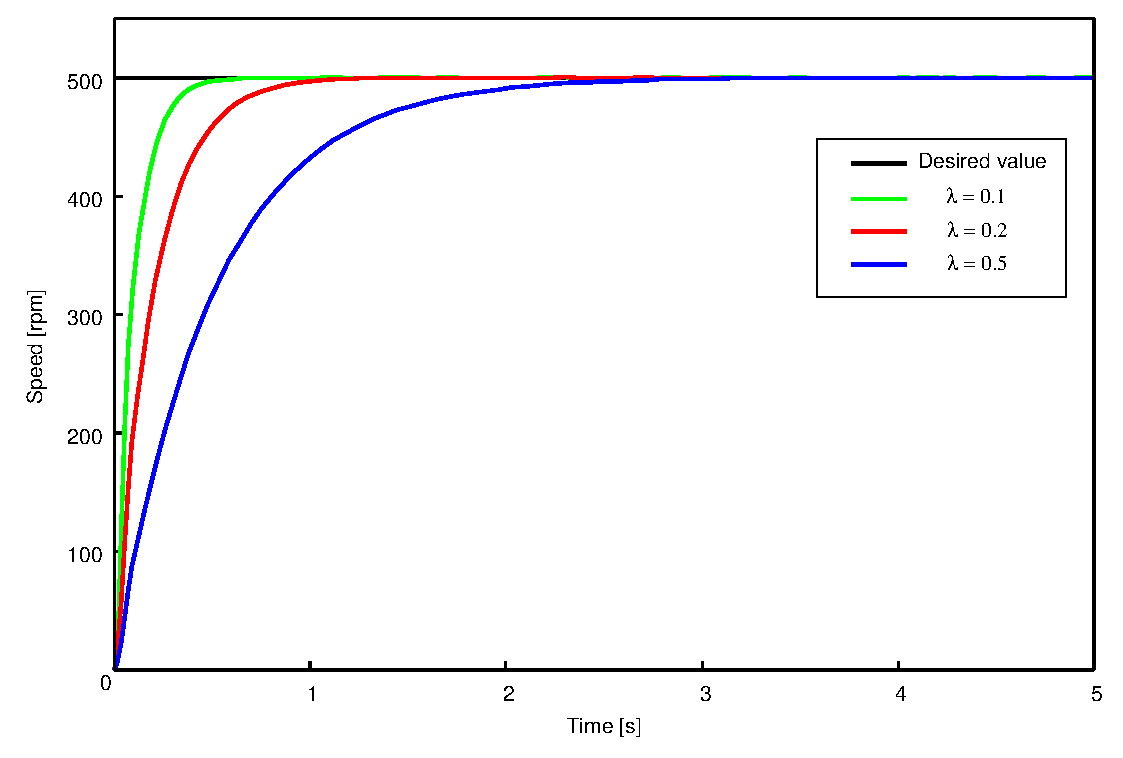
\includegraphics[width = 150mm]{fig/IMC_result.eps}
 \end{center}
 \caption{IMC法で$\lambda=0.1,0.2,0.5$として設計したシステムのステップ応答}
 \label{fig:IMC_result}
\end{figure}
%
%
\begin{figure}[tbp]
 \begin{center}
  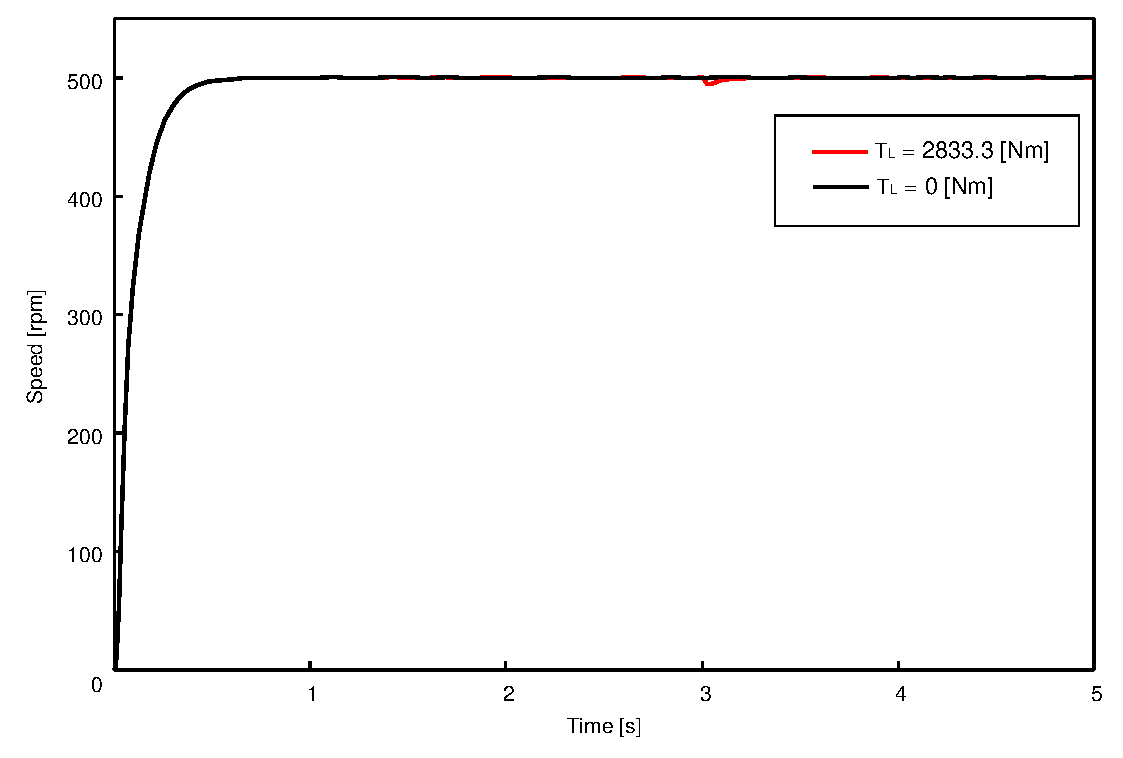
\includegraphics[width = 150mm]{fig/IMC_TL.eps}
 \end{center}
 \caption{IMCフィルタの係数$\lambda=0.1$としたときのステップ応答(負荷トルク$T_L=2833.3$)}
 \label{fig:IMC_TL}
\end{figure}
%
%
\begin{figure}[tbp]
 \begin{center}
  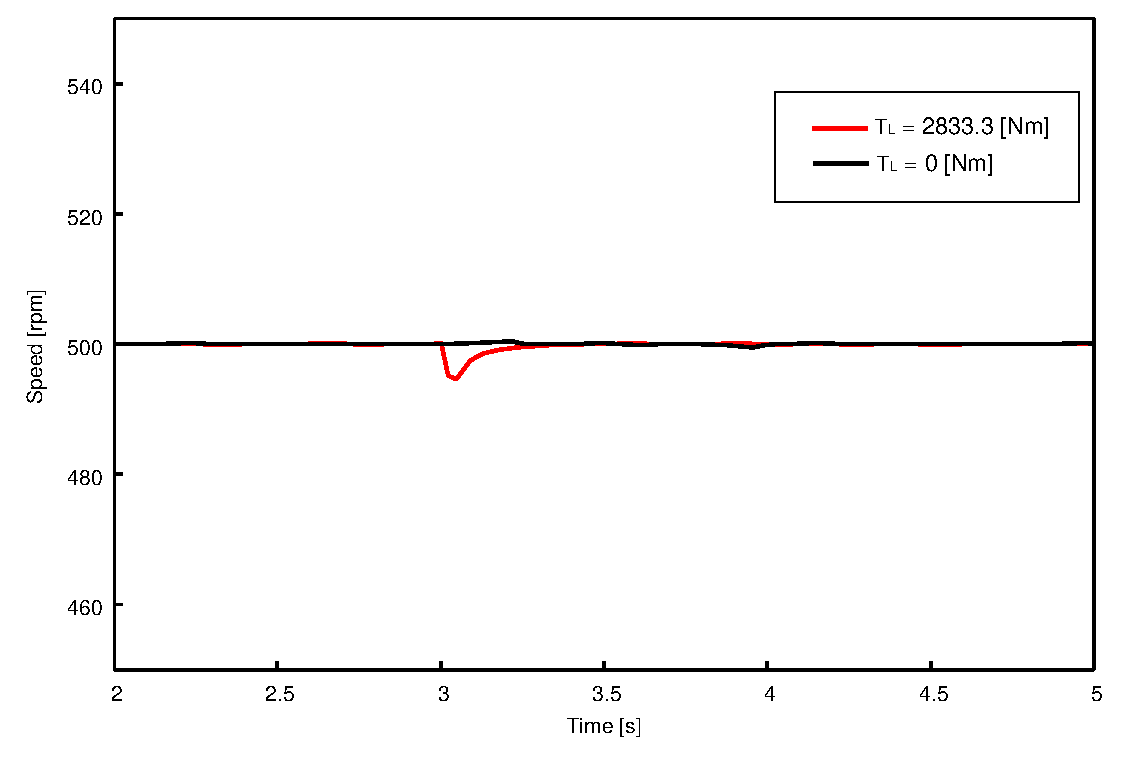
\includegraphics[width = 150mm]{fig/IMC_TLb.eps}
 \end{center}
 \caption{図\ref{fig:IMC_TL}の拡大図}
 \label{fig:IMC_TLb}
\end{figure}
%
図\ref{fig:IMC_result}を見ると$\lambda$の値が小さければ小さいほど早く目標値
に収束していることがわかる.即応性を高くするにはIMCフィルタの$\lambda$を
小さくすれば良いと考えられる.しかし,早く目標値に収束するためには,大きなトルク
を出力しなければならないので,出力トルクがモータの定格トルクを超え,モータが破壊しな
いように適切に$\lambda$を設定する必要があると考えられる.また,IMC法はプ
ラントのモデルの同定精度によって大きく制御系の性能が変わってくる.プラン
トのモデルを精度よく同定さえすればIMCフィルタの$\lambda$を調節すれば良い
ので制御系を容易に構成できると考えられる.
%
%%%%%%%%%%%%%%%%%%%%%%%%%
\section{まとめ}
%%%%%%%%%%%%%%%%%%%%%%%%%
I-PD制御,内部モデル制御を用いてDCモータの速度制御系を設計した.
%
\begin{thebibliography}{99}
\addcontentsline{toc}{section}{参考文献}

 \bibitem{denki} T.Sakamoto,
		 "Lecture Notes of Advanced Electrical Drive Control System",
		 2016.

 \bibitem{mecha} 坂本哲三,"電気機器の電気力学と制御", 森北出版, 2007.

 \bibitem{wakaru} 川田昌克,西岡勝博,"MATLAB/Simulinkによるわかりやすい
		 制御工学", 森北出版, 2001.

 \bibitem{kitamori} 北森俊行,"最適な制御系設計法と各種制御方式
		 の基礎・理論・応用の実際",アイ・エヌ・ジー,1993.

\bibitem{jiten} 足立修一ら,"制御の事典",朝倉書店,2015.

 \bibitem{kitamoripaper} 北森俊行,"IP-D制御方式の原理と設計法",システ
		 ム/制御/情報,Vol.42,No.1,pp.7-17,1998.
		 
\end{thebibliography}

\end{document}
